\documentclass[11pt]{article}
\usepackage{graphicx}
\usepackage{lipsum}
\graphicspath{ {images/} }
\begin{document}

\begin{titlepage}

\begin{center}
\begin{huge}
Swarm Visualiser - COS 301 Main Project
\\
Testing Specifications
\begin{small}
\\
Team: Dragon Brain
\\
Members:
\\
Matheu Botha u14284104
\\
Renton McInytre u14312710
\\
Emilio Singh u14006512
\\
Gerard van Wyk u14101263

\end{small}

\end{huge}
\end{center}
\end{titlepage}

\pagebreak

\tableofcontents

\pagebreak
\section{Frameworks and Mechanisms}
For our project, we are making use of Google Tests, a cross-platform Unit Testing library for C++. This is largely because our chosen standardised IDE, Jetbrains CLion has integrated support for the framework.

\section{Testing Strategies}

\subsection{Unit Tests}
Our project's unit tests work primarily based on Assert-like mechanisms for Google Test, wherein we generate objects with particular data and assure that values are as they should be, and ensuring invalid states are properly detected. These are done using the Google Test EXPECT keyword macros.
\newline Each test is defined within a TEST macro and can be run either individually or all together, via CLion. 


\section{Integration Tests}
\paragraph{•}
This section of the testing manual will contain all of the necessary details pertaining to the area of Integration Tests, and Integration Testing, as per project requirements and project dictates.
\subsection{Integration Requirements}
\paragraph{•}
In terms specifying the Integration Requirements for the project, we identify Program Modules. These Modules are separate components that will each provide services and possibly make use of other services from other Modules. As an integration challenge, the task is to ensure that all of these Modules are able to realise their service contracts and do not contribute to the failure of service contracts of other Modules.

The Modules are:
\begin{itemize}
\item Graphics Pipeline: The Graphics Pipeline will be required to integrate with the Manager and Data Models Module. This integration will take the form of message passing,System Snapshots, which are consumed by the Pipeline as provided by the Manager. The Graphics Pipeline similarly affects the User Interface. The Graphics Pipeline will then make use of the system snapshot in order to render, on the User Interface, the implications realised internally by the General Optimiser.
\item General Optimiser: The General Optimiser will produce System Snapshots which will be stored in Data Models inside the Manager Module. This General Optimiser, by the use of Settings Package, will then be configured to meet specific user requirements. 
\item User Interface: The User Interface is going to communicate with the Manager Module. The user changing system parameters, or configuring them, will generate Settings Package objects and these will be sent to the Manager for use in adjusting configurations. The User Interface will also be receiving, and rendering, message packets from the Graphics Pipeline. These packets will result in new visual information being displayed to the user.
\item Manager: The Manager Module will be the core and most important part of Integrating the Modules of the system. All of the other Modules will have to perform some manner of interaction with the Manager which will then perform some other form of interaction, on their behalf,to other Modules. This connectivity between all of the other Modules and this one, means that in order to successfully integrate the System Modules, we will require a Manager component that is capable of relaying, creating and receiving messages from all of the other System Modules.

\end{itemize}
 
\subsection{Strategies}
\paragraph{•}
The general integration strategy will be to construct the Manager Module and then perform unit testing of it by creating fake objects/service requests and determining if the Manager Module is able to contractually fulfil those service requests and create the required objects/class instances as per need. Once this process has been finished, the next step will be to construct the actual Modules that communicate with the Manager and then perform testing where the test objects request services from the Manager and the Manager must again provide to these real objects, the requirements of the service contracts that bind them. Once this is completed, the final stage of the integration testing will require a stress testing component in order to identify system weaknesses in optimisation that would affect the performance of the system of a whole under serious load. This can only be determined by subjecting the system to higher-than-normal workloads which will have the effect of identifying the most stress-failure prone areas of the system.

\section{Areas of Major Concern}
In terms of Areas of Concern, these can be defined within a number of potential Key Points of Failure within the Project. These can be split into subsections based on the Modules within the project.
\subsection{Graphics Pipeline and General Optimiser}
One of the major performance concerns of the project can be translated into a potential point of failure. This is the potential for either the Graphics Pipeline or the General Optimiser to work faster than the other, leaving the other part of the system waiting (or spinning) until the other provides work to complete. Theoretically, failure could occur if this situation is not handled correctly and the Graphics Pipeline attempts to access a Snapshot from the Queue which does not exist, or the General Optimiser attempts to add a Snapshot when the Queue is full (ie the Heap is full). 
\newline To cover for this, tests must be run that ensure that both sub-systems are capable of correctly handling such situations by spinning until the Queue's state has changed.
\subsection{User Interface}
With regards to the User Interface, this is where potential for human error can occur at runtime. Theoretically a user will only submit relevant data via the User Interface, however it is not impossible that a user will accidentally enter some kind of invalid data. This would naturally cause problems for the entire system.
\newline Thus, extensive testing must be done to ensure that the SettingsPackage generated does not have invalid data within and the system should attempt to correct any failures that occur.


\section{Example Unit Test}
\paragraph{•}
Following is an example of a Test in the general SettingsPackage, using Google Tests.
\begin{figure}[h]
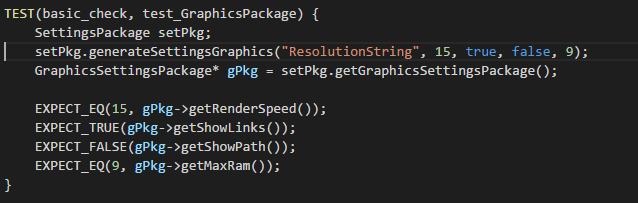
\includegraphics[scale=0.7]{GTest.png}
\end{figure}

\end{document}
